% Intended LaTeX compiler: pdflatex
\documentclass[11pt]{article}
\usepackage[utf8]{inputenc}
\usepackage[T1]{fontenc}
\usepackage{graphicx}
\usepackage{grffile}
\usepackage{longtable}
\usepackage{wrapfig}
\usepackage{rotating}
\usepackage[normalem]{ulem}
\usepackage{amsmath}
\usepackage{textcomp}
\usepackage{amssymb}
\usepackage{capt-of}
\usepackage{hyperref}
\author{Harriet Sands \& Hillary Juma}
\date{}
\title{It takes a village\\\medskip
\large Data Science Campus @ONS}
\hypersetup{
 pdfauthor={Harriet Sands \& Hillary Juma},
 pdftitle={It takes a village},
 pdfkeywords={},
 pdfsubject={},
 pdfcreator={Emacs 26.3 (Org mode 9.3)}, 
 pdflang={English}}
\begin{document}

\maketitle
\section*{My Career}
\label{sec:orge012aa5}
Harriet Sands
\section*{}
\label{sec:org4847d18}
\begin{NOTES}
\end{NOTES}

\section*{}
\label{sec:org1949e62}
\begin{center}

\includegraphics[width=.9\linewidth]{./img/pydata.png}
\end{center}
\begin{center}

\includegraphics[width=.9\linewidth]{./img/hm-gov-logo.png}
\end{center}
\begin{center}

\includegraphics[width=.9\linewidth]{./img/datakind.png}
\end{center}

\section*{}
\label{sec:org4f73c2a}
We apply data science
and build skills
for public good
\begin{NOTES}
We work at the frontier of data science and AI:
\begin{itemize}
\item building skills and applying tools, methods and practices – to create new understanding and improve decision-making for public good.
\end{itemize}

We define data science as:
\begin{itemize}
\item Applying the tools, methods and practices of the digital and data age to create new understanding and improve decision-making.
\end{itemize}

The goals of ONS’s Data Science Campus are:
\begin{itemize}
\item to investigate the use of new data sources, including administrative data and
big data for public good
\item to help build data science capability for the benefit of the UK
\end{itemize}
A new generation of tools and technologies are used to exploit the growth and
availability of these new data sources and provide rich informed measurement and analyses on the economy, the global environment and wider society.
\end{NOTES}
\section*{}
\label{sec:org9ae9f63}
\section*{}
\label{sec:orgd0981c3}
\begin{center}
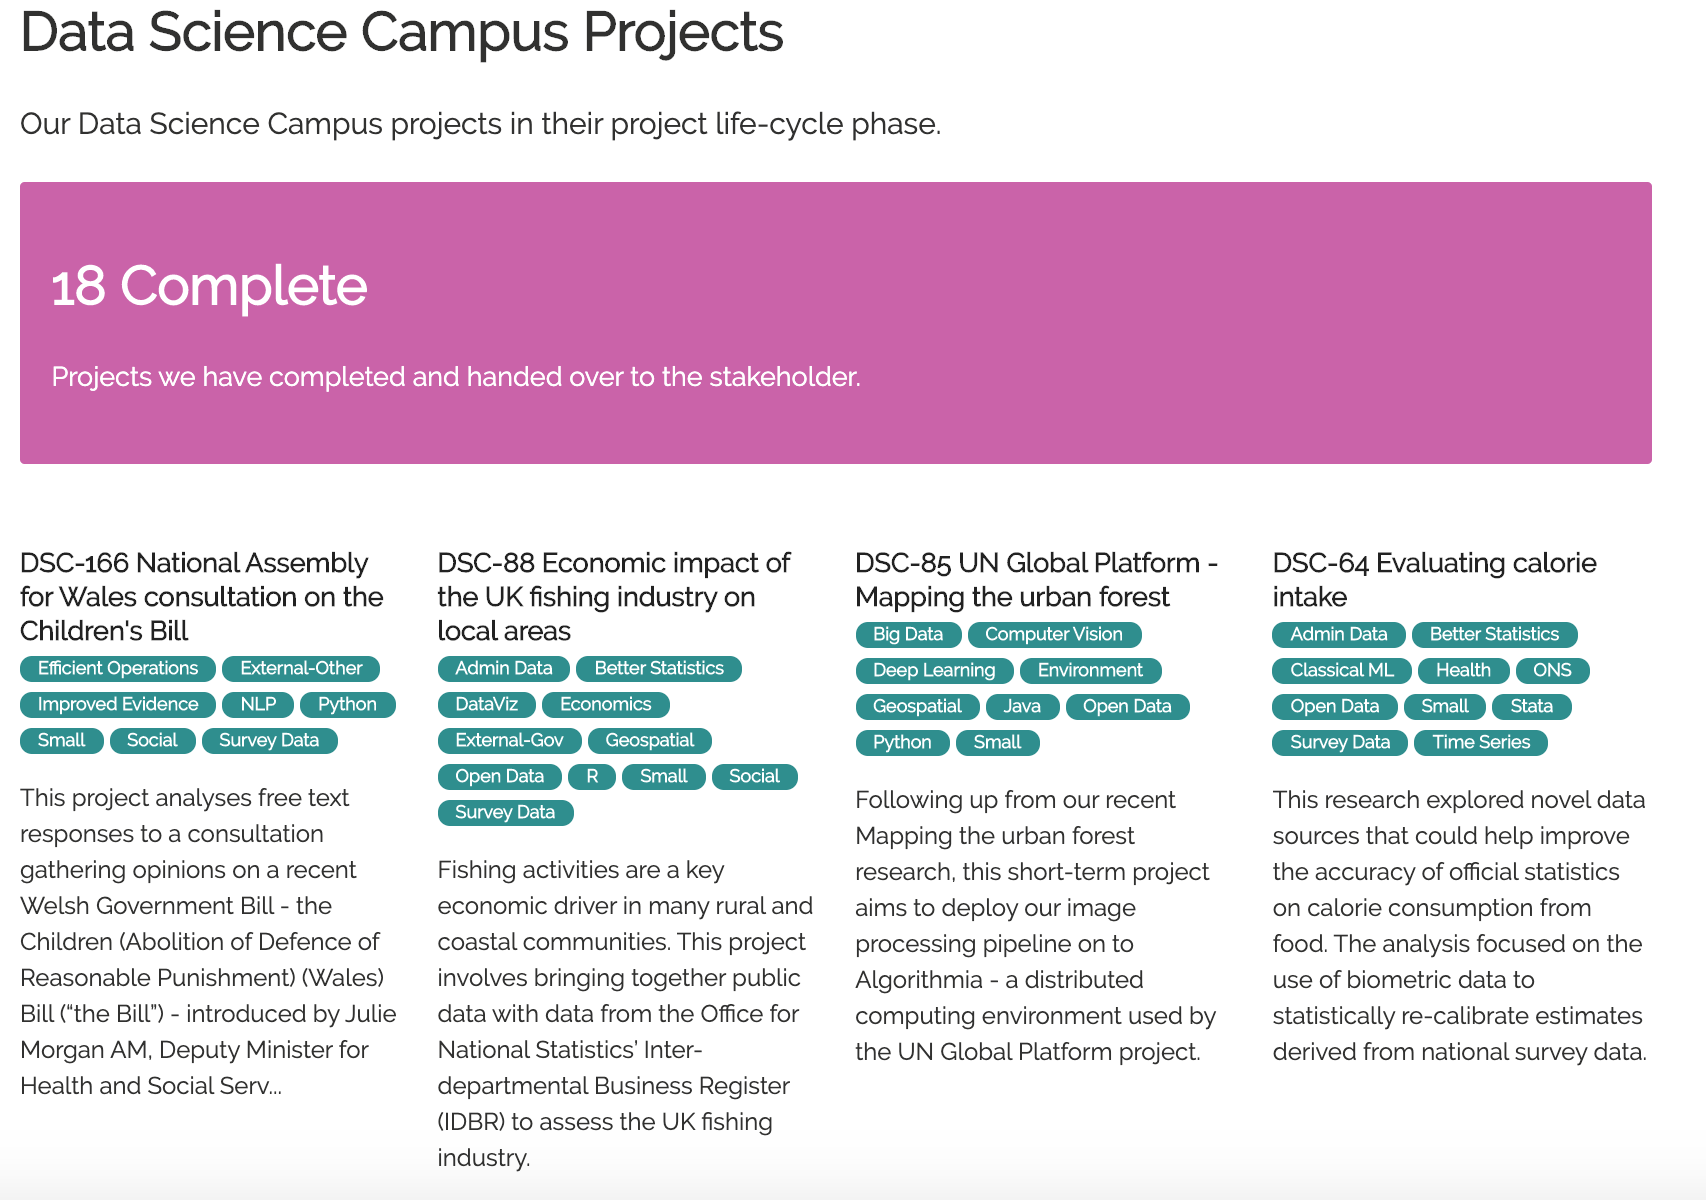
\includegraphics[width=.9\linewidth]{./img/dsc-projects.png}
\end{center}
*
MDataGov
Data Science Accelerator
DSC courses:
\begin{itemize}
\item Fundamentals of Data Science
\end{itemize}
\begin{itemize}
\item The Art of the Possible
\end{itemize}
\end{document}
